\section{Mechanisms Overview}

\begin{frame}
	\frametitle{Outline}
	\begin{tcolorbox}[coltitle=yellow!50!black,colframe=magenta!25,split=.2,title=Mechanism Components]
		Freedoms, Constraints, and Mobility.
		\tcblower
		%\begin{itemize}
		 Kinematic Geometry: Pairs, linkages, and mechanisms.
		 \vspace{.2cm}
		\newline
		Motion of linkages: Screws, and spatial motions.
		\vspace{.2cm}
		\newline
		Freedom and Mobility: Freedoms, unfreedoms, connectivity, mobility;
		\vspace{.2cm}
		\newline
		Gr{\"u}bler-Kutzbach's mobility criterion and examples.
	\end{tcolorbox}
\end{frame}
 
\begin{frame}
	\frametitle{Definition of a Mechanism}
		\begin{definition}[Author's Definition]
			A \textcolor{blue}{connection} of  mechanical, magnetic, electrical, hydraulic, or pneumatic components forming an \textcolor{magenta}{assemblage}, meant for moving rigid, semi-rigid or non-rigid bodies via a \textcolor{green}{controlled generation} of (sometimes) \textcolor{red}{motion}.
		\end{definition}
		%
	\begin{tcolorbox}[coltitle=red!80!black,colframe=magenta!25,title=Kenneth Hunt (1978)]
			A means of \textit{transmitting}, \textit{controlling}, or \textit{constraining} the relative movement.
	\end{tcolorbox}
\end{frame}

\begin{frame}
	\frametitle{Mechanisms}
	\begin{block}{Joints and links}
		Joints are a result of the connecting points between rigid links.
		Links may be rigid mechanical parts, elastic, (vulcanized) rubber components, diaphragms, conveyor belts, spring-damper systems e.t.c.
	\end{block}
	%	
	\begin{block}{Rigid Mechanism}
		Our chief focus will be rigid links, \textcolor{red}{pairs}, components and mechanisms in general.
	\end{block}
\end{frame}


\begin{frame}
	\frametitle{Mechanisms Examples}
	\begin{tabular}{|c|c|} 
	%
	\hline  \\
	Spring-Mass-Damper System & Excavator \\
	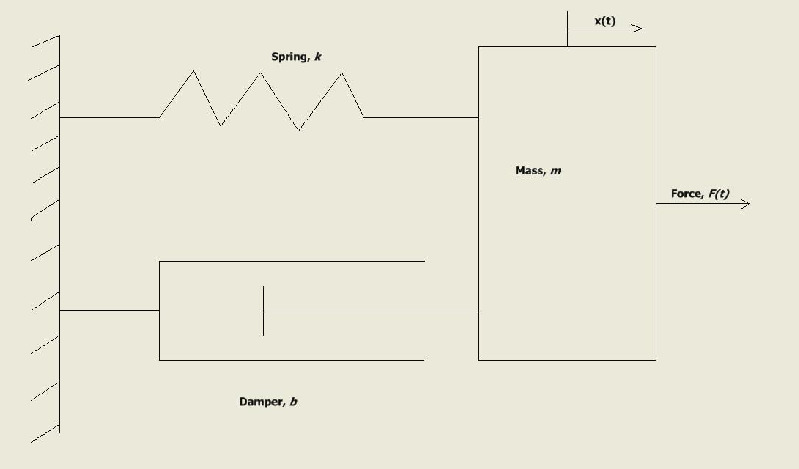
\includegraphics[height=5em,width=10em]{figures/spring-mass-damper.jpg} & 
	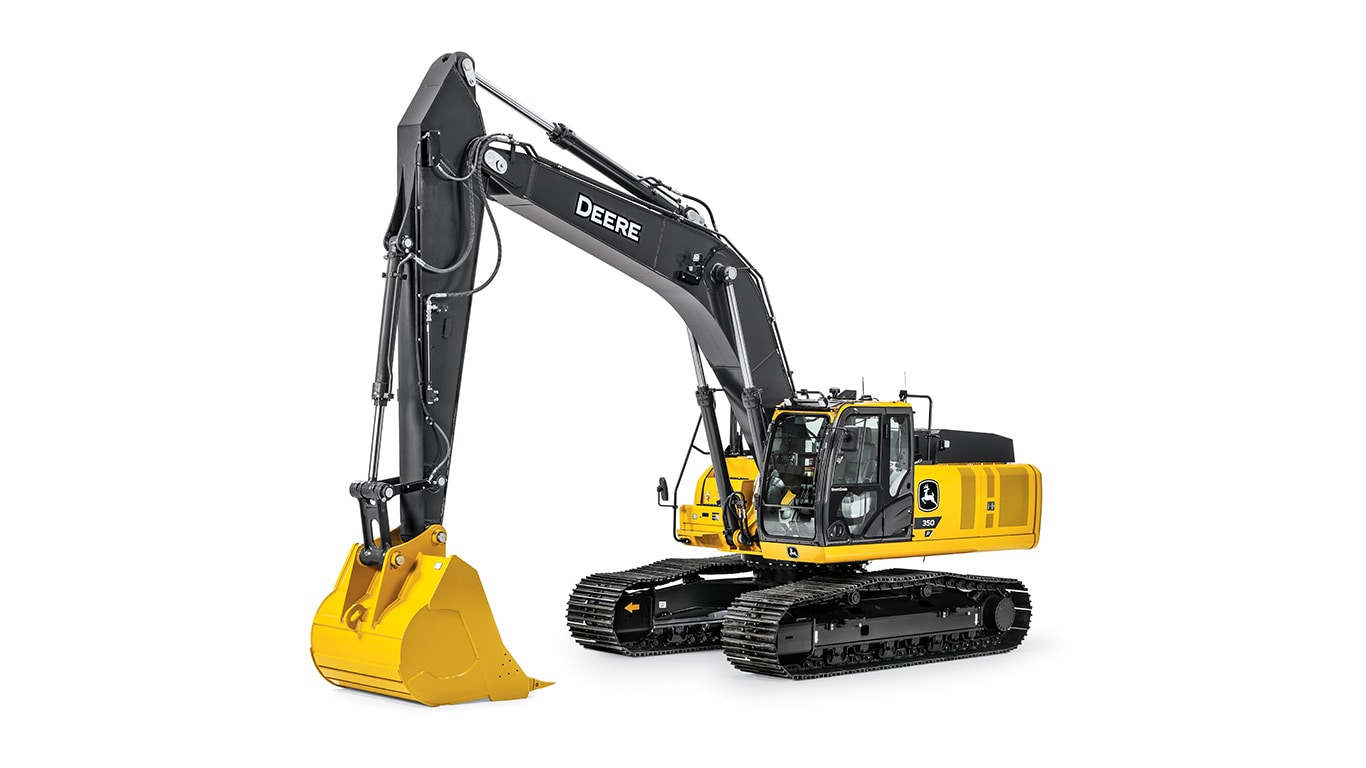
\includegraphics[height=5em,width=10em]{figures/excavJohnDeere.jpg} \\
	\hline \\
	Car suspension & Daimler  Plant \\
	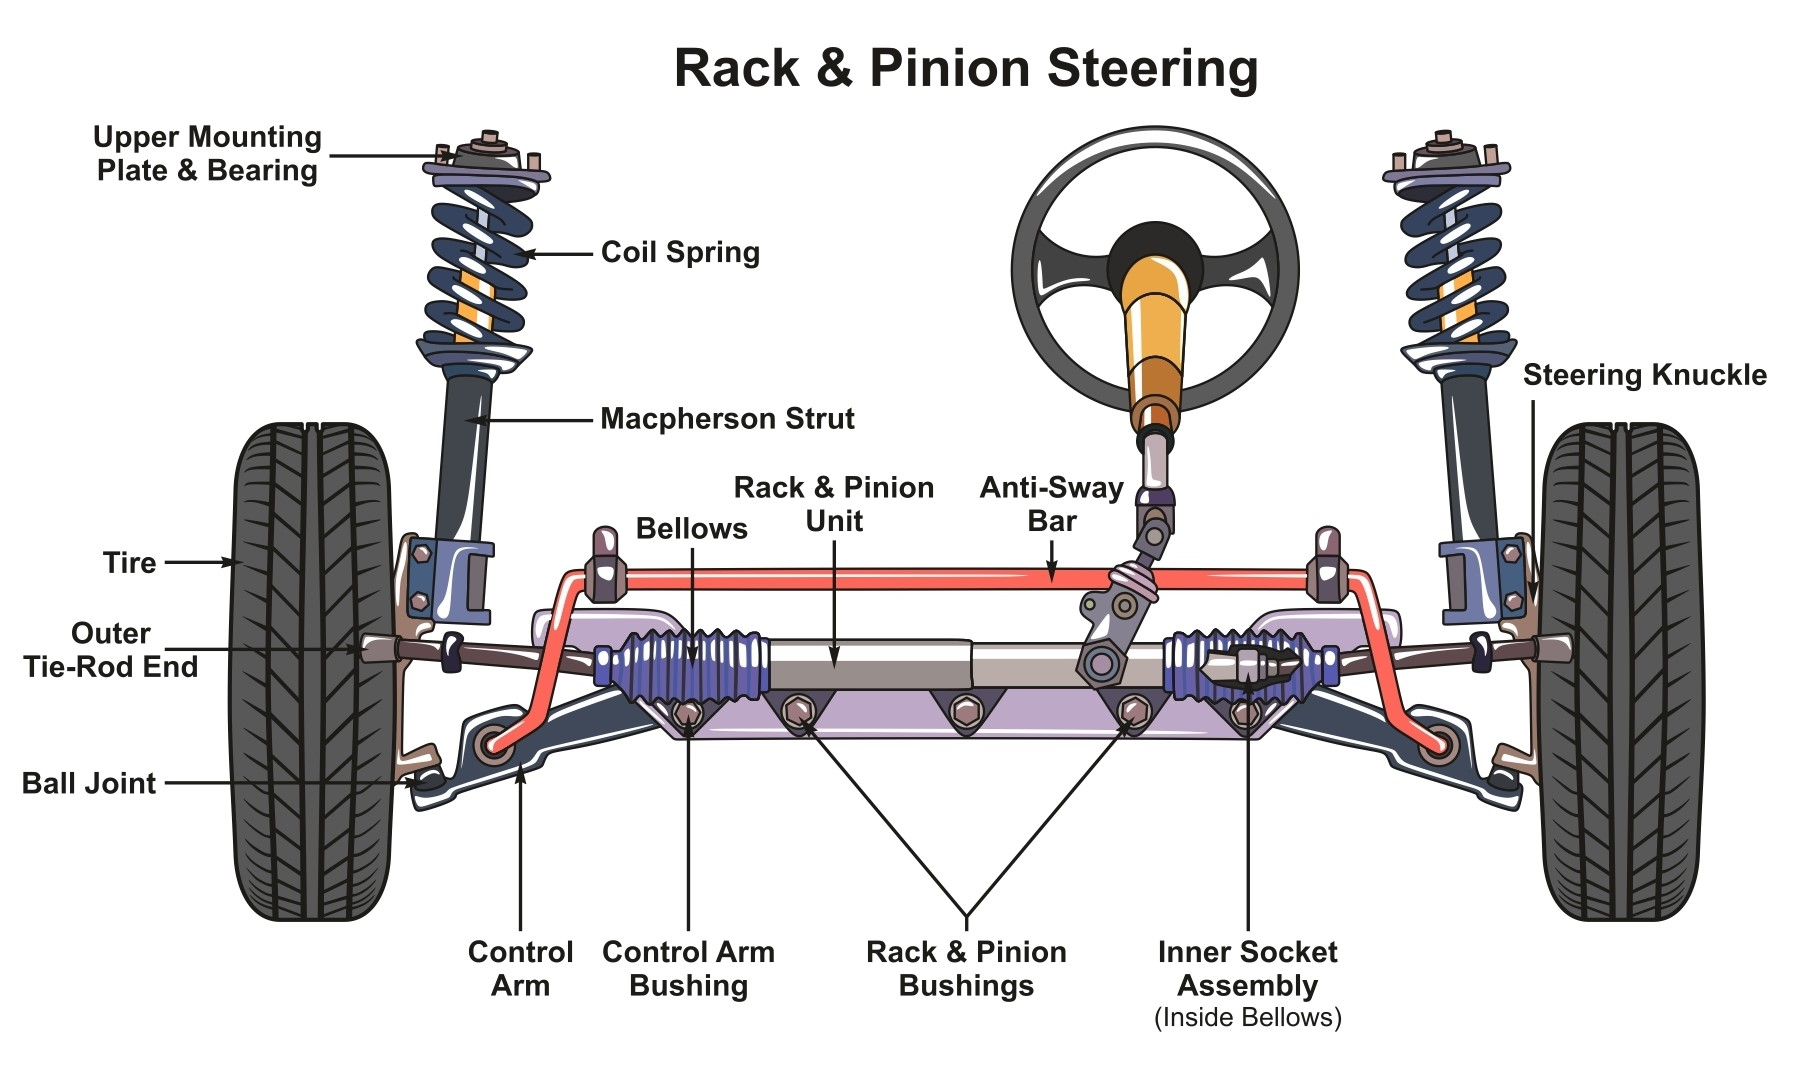
\includegraphics[height=5em,width=10em]{figures/carsusp.jpg} &
	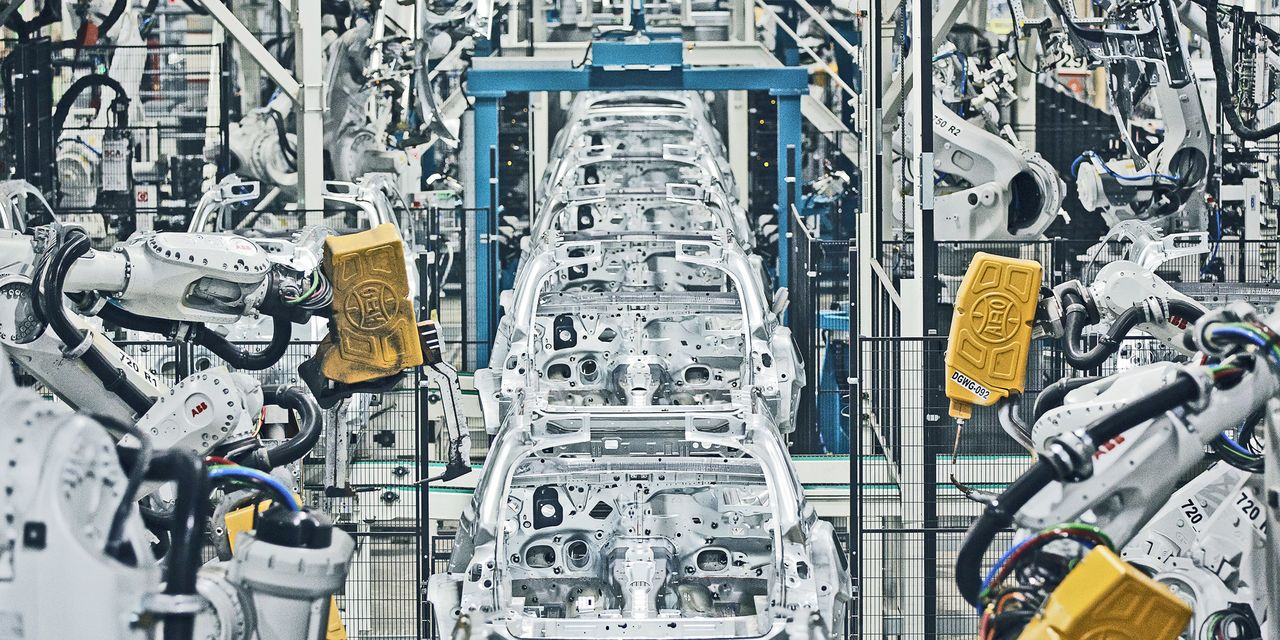
\includegraphics[height=5em,width=10em]{figures/daimler_manuf.jpeg} \\
	\hline
	\end{tabular}
\end{frame}


\begin{frame}
	\frametitle{Open Kinematic Chains}
	%	
	\begin{block}{Chains}
		Open kinematic chains are based off the anthropomorphic construction of the human hand with cantilevered beam structures.
	\end{block}
	\begin{block}{Chain Mechanisms and Error Amplification}
		Amplifies errors from waist (or base frame) all the way to the tool frame. Control difficult. 
	\end{block}
	%
	\begin{block}{Control}
		Feedforward control: High power and precision hydraulic actuators for servo motors. \\
		Sensory feedback control: Force sensing (Ernst, 1962). 
	\end{block}
\end{frame}


\note{The PUMA arm is the world's first serial kinematic chain. Developer: Victor Scheinman, Stanford student in the `50's. Made several iterations. Patent Rights: Joe Engelberger, (Danbury Unimation, 1961). Joe -- father of robotics -- created world's first robotics company in '61.}
\begin{frame}
	\frametitle{Open Kinematic Robot Mechanisms}
	\begin{definition}[Ken Salisbury Jr., 1982]
		``\footnotesize \textit{[Robots are] our fascination with constructing mechanical analogues of ourselves... [this fascination] has led us to place all sorts of hopes and expectations in robot capabilities}."
	\end{definition}
	\begin{columns}[t]
		\begin{column}{5cm}
			\begin{minipage}[b]{.5\textwidth}
				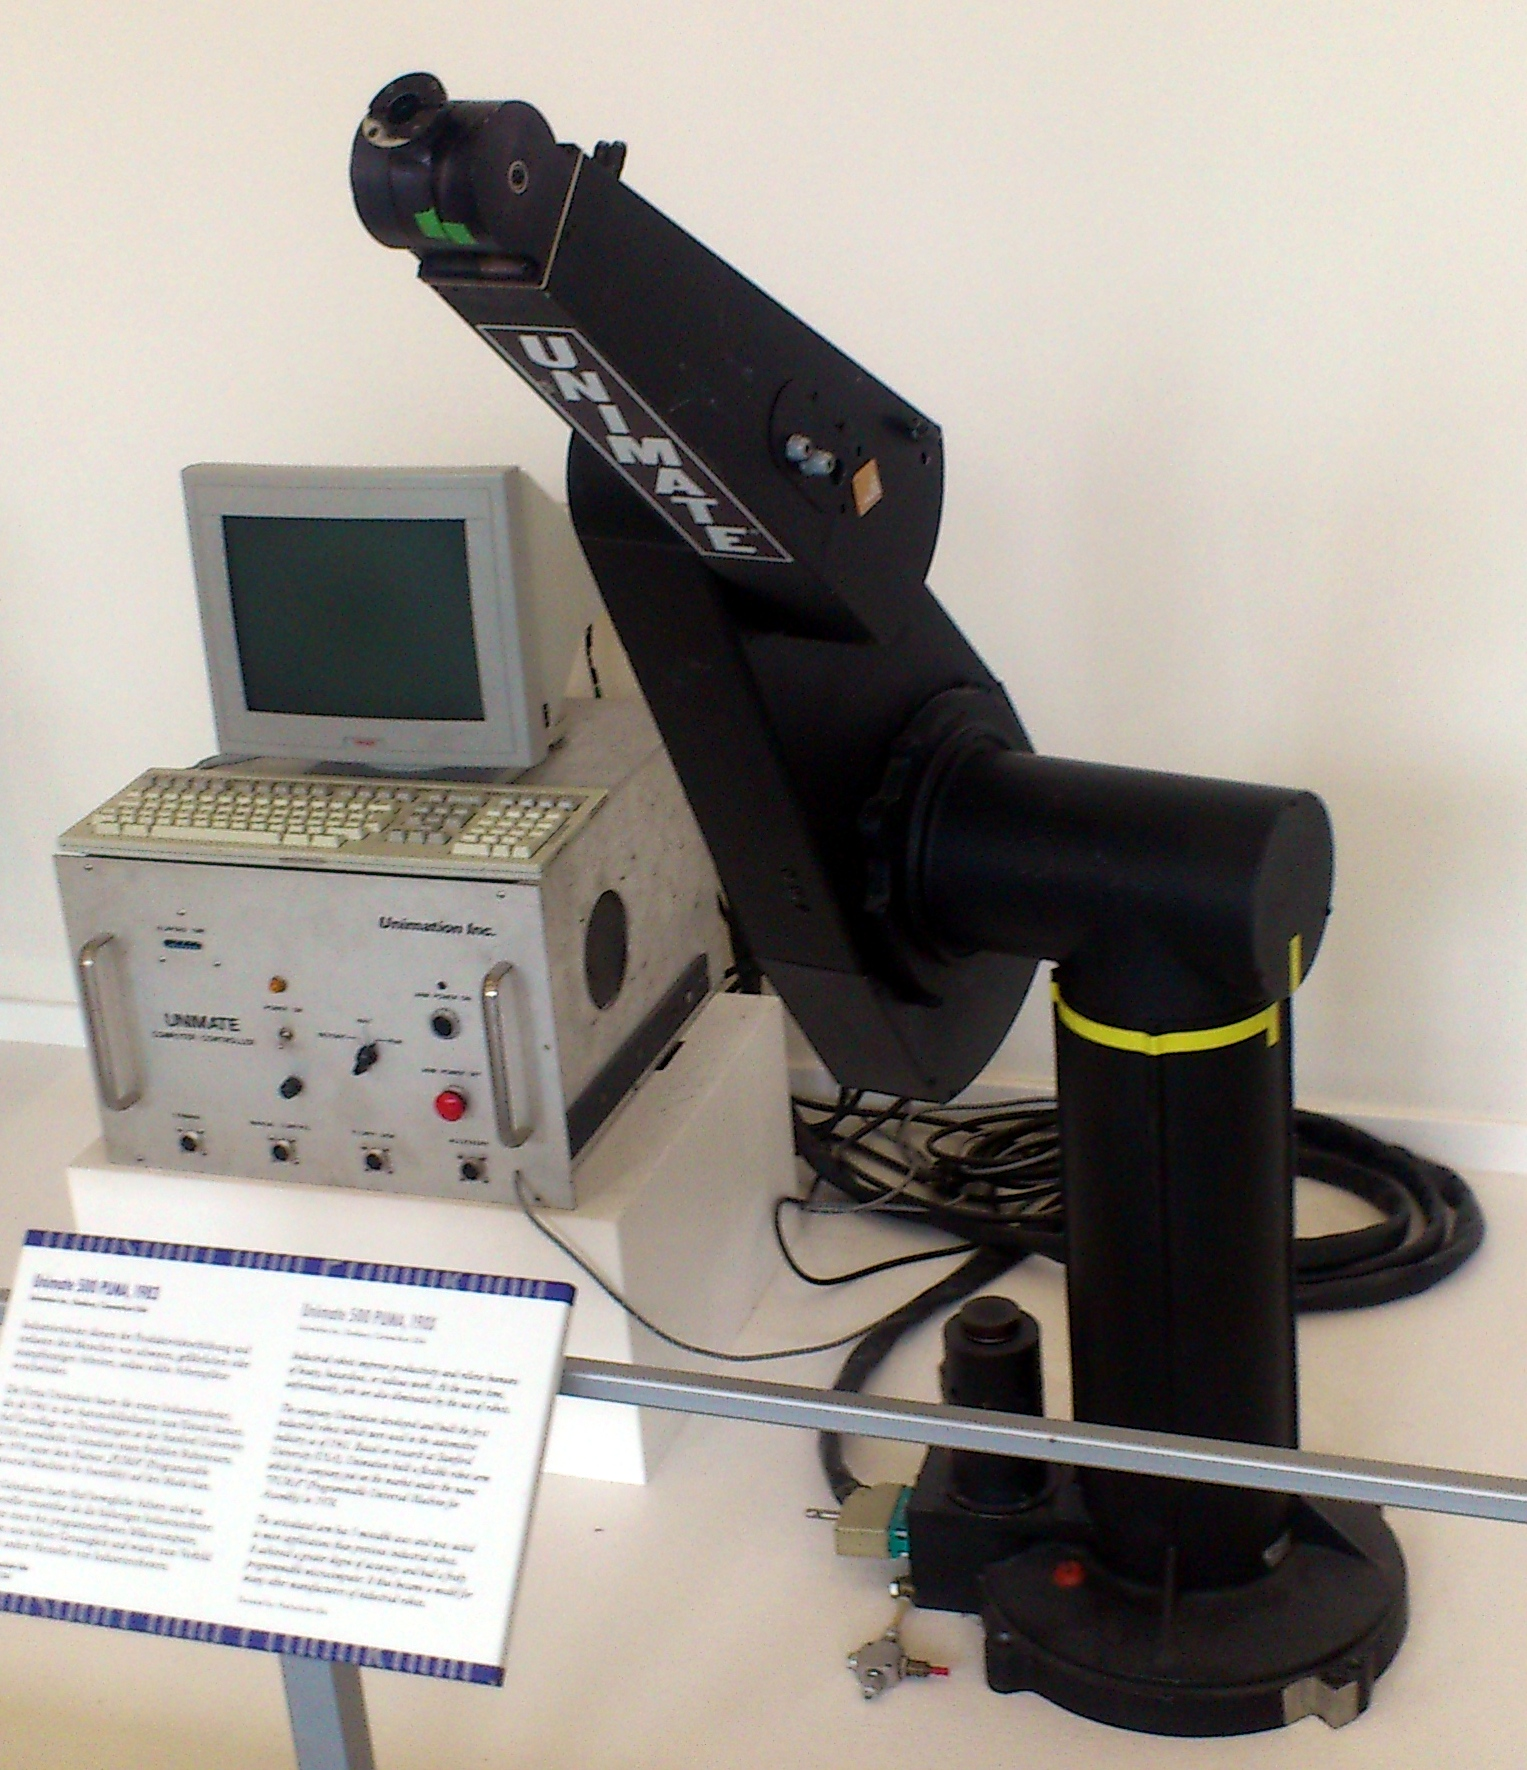
\includegraphics[width=1.5\textwidth, height=1.5\textwidth]{../Notes/figures/PUMA.jpg} \\
				\footnotesize{The St{\"a}ubli PUMA Robot (1956).} %Programmable Universal Manipulation Arm.}
		\end{minipage}
		%
	\end{column}	
	\begin{column}{5cm}
		\begin{minipage}[b]{.5\textwidth}
			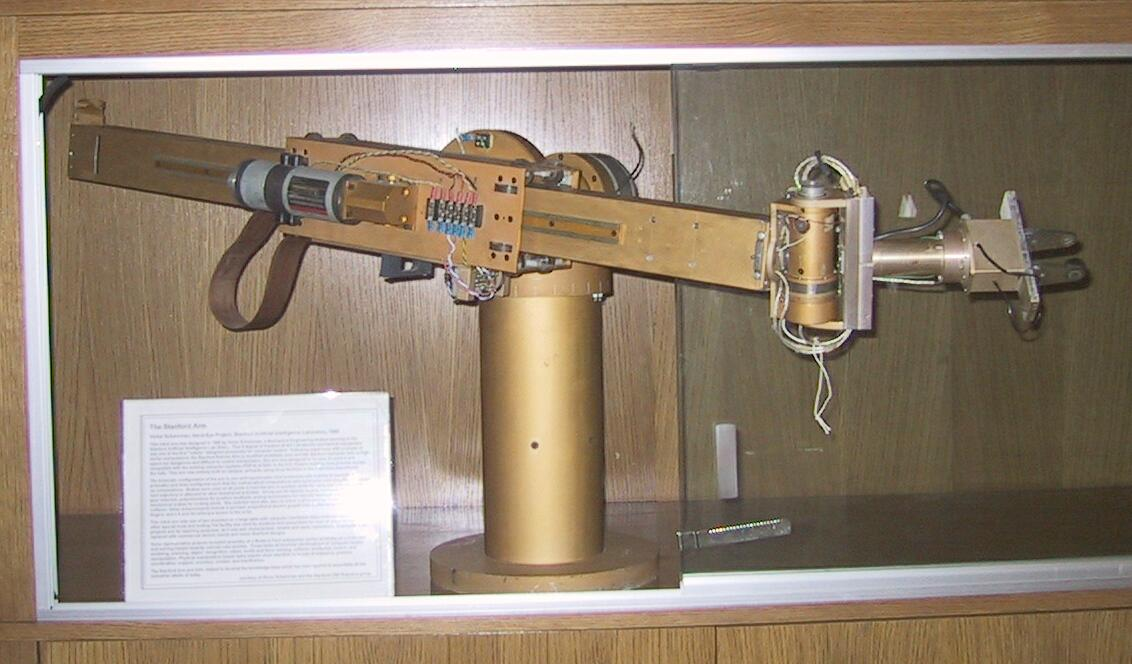
\includegraphics[width=1.5\textwidth, height=1.5\textwidth]{../Notes/figures/StanfordArm.jpg}  \\
			\footnotesize The Stanford Arm (Infolab 1969). %Six degrees of freedom open kinematic chain.
		\end{minipage}
	\end{column}
\end{columns}
\end{frame}

\begin{frame}
	\frametitle{Open Kinematic Chains}
	%
	\begin{tcolorbox}[coltitle=blue!80!yellow,colframe=brown!80]
		Open kinematic chains provide unstructured environmental interaction.
	\end{tcolorbox}
	\begin{tcolorbox}[coltitle=blue!80!yellow,colframe=gray!100]
		Project MAC, MIT.
	\end{tcolorbox}
	\begin{tcolorbox}[coltitle=blue!80!yellow,colframe=black!80]
		Tomovic and Boni's pressure sensed grasp.
	\end{tcolorbox}
	\begin{tcolorbox}[coltitle=blue!80!yellow,colframe=pink!100]
		Binary robot vision system (McCarthy et al, 1963).
	\end{tcolorbox}
\end{frame}

\begin{frame}
	\frametitle{Open Kinematic Chains}
	%
	\begin{tcolorbox}[coltitle=cyan!80,colframe=green!100]
		Stanford Manipulator.
	\end{tcolorbox}
	\begin{tcolorbox}[coltitle=blue!80!yellow,colframe=blue!100]
		Boston arm.
	\end{tcolorbox}
	\begin{tcolorbox}[coltitle=blue!80!yellow,colframe=red!100]
		The AMF (American Machines and Foundry) arm.
	\end{tcolorbox}
	\begin{tcolorbox}[coltitle=blue!80!yellow,colframe=yellow!100]
		General electric's walking robot (1969).
	\end{tcolorbox}
\end{frame}


\begin{frame}
	\frametitle{Long Walk Towards Direct Drive Robot Arms}
	
	\begin{tcolorbox}[coltitle=magenta!80!green,colframe=yellow!80!green]
		The 50's, 60's nd 70's witnessed use of hydraulics  for (feedforward) position control.
	\end{tcolorbox}
	
	\begin{tcolorbox}[coltitle=magenta!80!green,colframe=blue!80!green] 
		For feedback control, force sensors and pressure sensors were used in closed-loop scenarios.
	\end{tcolorbox}

	\begin{tcolorbox}[coltitle=magenta!80!green,colframe=red!80!green] 
		Electrical actuation meant that robots had to be operated at high speeds. Needs for gear reduction for safe operations at low speeds. 
	\end{tcolorbox}

	\begin{tcolorbox}[coltitle=magenta!80!green,colframe=brown!80!green]
		 With gear reduction came backlash, friction, and associated expenses.
	\end{tcolorbox}
\end{frame}


\note{CMU DD I/II Arms: Workspace is donut shaped. OD:  90cm; ID: 21.7cm; $1.8m^2$ workspace area. Built by Harry Asada. Structural design similar to aircraft gimbal arm; Uses Samarium Cobalt rare earth magnet brushless DC motors on first 3 joints, and AlNiCo magnets on tip joints. No belts, transmissions making for faster transmitting of motions, less friction, low energy, low compliance. Each joint has complex AL housing which enables: (i) Control of geometrical relationships of bearing assembly; (ii) Control of servo components to bearing assembly; (iii) Controls of rotational axes to consecutive joints.}


\begin{frame}
	\frametitle{Direct Drive Robot Mechanism: CMU DD I Arm}
	\begin{tcolorbox}[coltitle=blue!80!yellow,colframe=brown!80!green]
		Along came Harry Asada.
	\end{tcolorbox}
	\begin{columns}[t]	
		%
		\begin{column}{.45\columnwidth}
			\begin{minipage}[b]{\textwidth}
				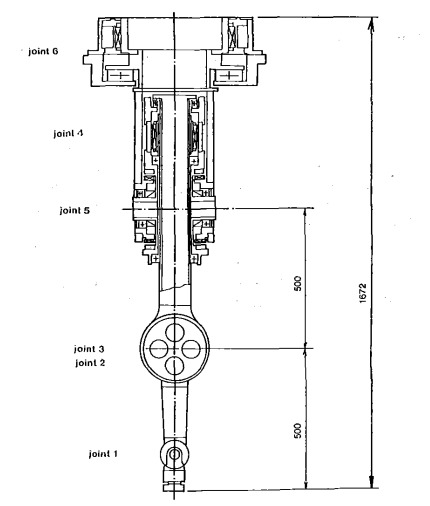
\includegraphics[width=1.2\textwidth, height=1.2\textwidth]{figures/cmu_arm.jpg} \\
				\footnotesize{Arm Schematics Transmission} %Programmable Universal Manipulation Arm.}
		\end{minipage}
		%
	\end{column}
	%
	\begin{column}{.45\columnwidth}
		\begin{minipage}[b]{\textwidth}
			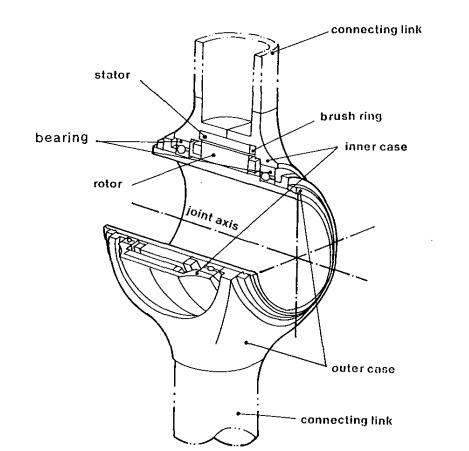
\includegraphics[width=1.2\textwidth, height=1.2\textwidth]{figures/dd_joints.jpg} \\
			\footnotesize{Joint schematic} %Programmable Universal Manipulation Arm.}
	\end{minipage}
	%
	\end{column}
\end{columns}
\end{frame}

\begin{frame}
	\frametitle{Direct Drive Robot Mechanism: CMU DD I Arm}
	\begin{columns}[t]					%
		%
		\begin{column}{.45\columnwidth}
			\begin{minipage}[b]{\textwidth}
				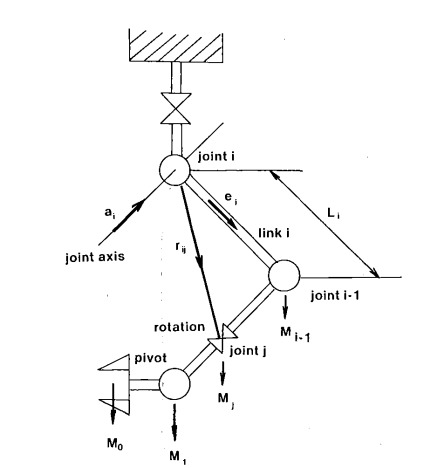
\includegraphics[width=1.1\textwidth, height=1.5\textwidth]{figures/dd_kinematics.jpg} \\
				\footnotesize{Kinematic model} %Programmable Universal Manipulation Arm.}
		\end{minipage}
		%
	\end{column}
	\begin{column}{.45\columnwidth}
		\begin{minipage}[b]{\textwidth}
			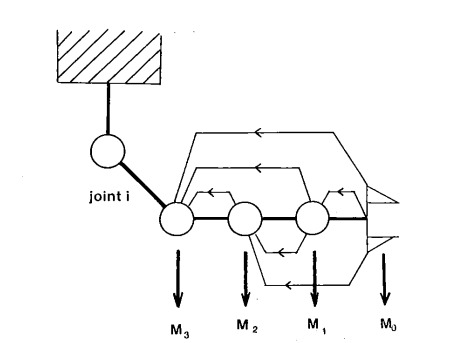
\includegraphics[width=1.2\textwidth, height=1.5\textwidth]{figures/dd_load_joints.jpg} \\
			\footnotesize{Errors Transmission} %Programmable Universal Manipulation Arm.}
		\end{minipage}
	\end{column}
	\end{columns}\end{frame}


\note{First direct-drive robot without a gearbox. Selective compliance in X-Y directions given its articulated jointed arms. One-freedom motion along $Z$ direction given its constrained arm New generations such as Cobra i600/i800 include power amplifiers, system and servo controls etc embedded in the robot's base. Kuka Scara arm: Lightweight, fast, powerful, low maintenance, energy consumption, investment costs etc.}
\begin{frame}
	\frametitle{SCARA Robot Mechanisms}
	\begin{columns}[t]	
		\begin{column}{5cm}
			\begin{minipage}[b]{.5\textwidth}
				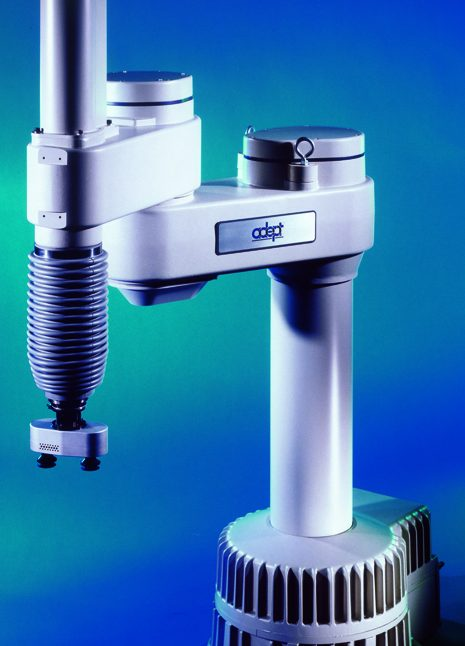
\includegraphics[width=1.5\textwidth, height=1.5\textwidth]{figures/adeptone.jpg}  \\
				\footnotesize The Adept One SCARA robot (Debuted 1984). 
			\end{minipage}
		\end{column}
		%
		\begin{column}{5cm}
			\begin{minipage}[b]{.5\textwidth}
				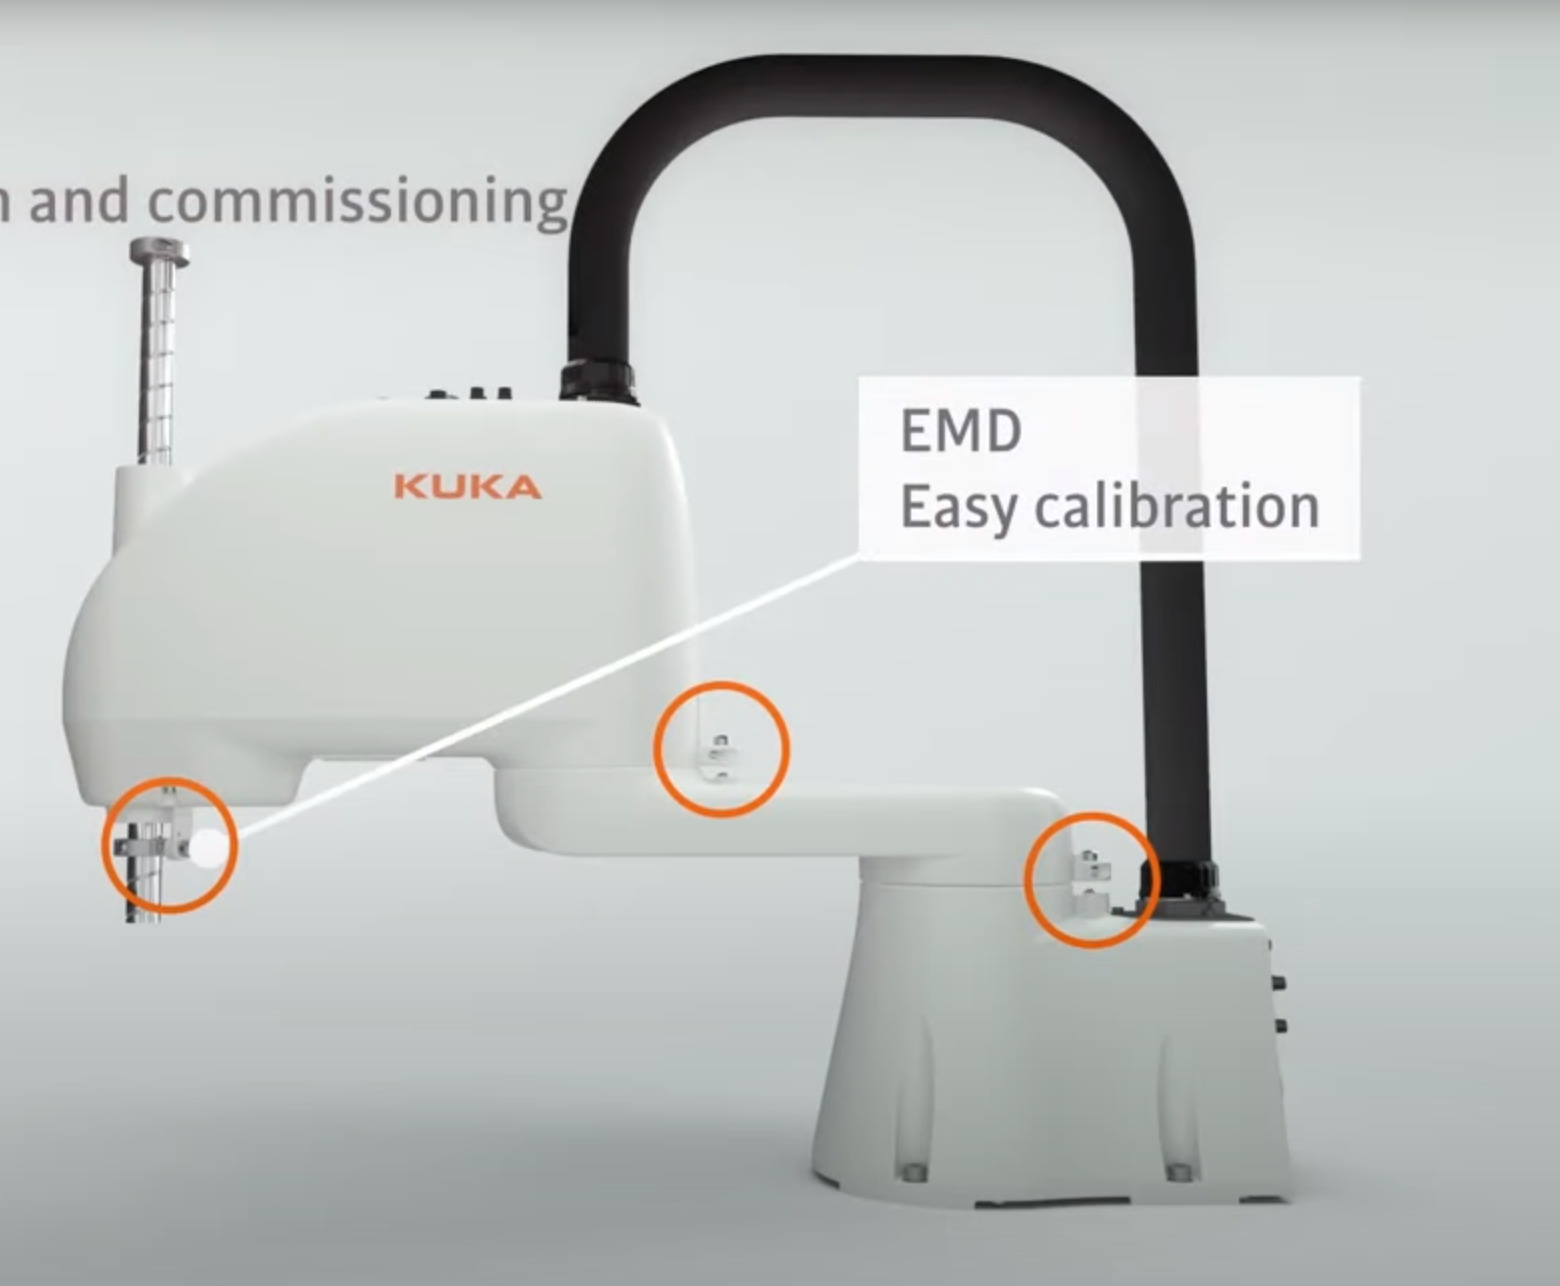
\includegraphics[width=1.5\textwidth, height=1.5\textwidth]{figures/Scara.jpg} \\
				\footnotesize{Kuka's SCARA arm, 2022. \copyright Kuka Robotics} %Programmable Universal Manipulation Arm.}
		\end{minipage}
		%
	\end{column}
\end{columns}
\end{frame}


\begin{frame}
	\frametitle{Serial mechanisms research in the 80's}
	%
	\tcbset{coltitle=cyan!80,colframe=gray!80!green,title=Mechanisms in the 80's,
		enlarge left by=-5mm,enlarge right by=0mm,width=\linewidth+5mm}
	\begin{tcolorbox}[toggle enlargement=none]
		With the 80's came the arrival of PCs. Lots of research went into computational algorithms for the kinematics and kinetics of (mostly) anthropomorphic robot arms.
	\end{tcolorbox}
	\begin{tcolorbox}[coltitle=magenta!70,colframe=blue!80!red,title=Active control schemes,toggle enlargement=forced]
		Efficient recursive Lagrangian and computational methods for the gravitational and Coriolis forces in Newton-Euler equations.
	\end{tcolorbox}
	\begin{tcolorbox}[coltitle=pink!70,colframe=gray!80!red,title=Feedback Linearization,toggle enlargement=evenpage]
		Dynamics feedback linearization for precise bounds on manipulator performance.
	\end{tcolorbox}
\end{frame}

\begin{frame}
	\frametitle{Serial mechanisms research in the 90's}
	%
	\tcbset{coltitle=pink!80,colframe=gray!80,title=Robotworld,
		enlarge left by=-5mm,enlarge right by=0mm,width=\linewidth+5mm}
	\begin{tcolorbox}[title=Automatix,toggle enlargement=none]
		Reconfigurable robots for various assembly ops.
	\end{tcolorbox}
	\begin{columns}[b]
		\begin{column}{.48\columnwidth}			
			\begin{tcolorbox}[colframe=blue!80!green, coltitle=white!80,toggle enlargement=none]
				First industrial-scale re-configurable robot and with machine vision components. RAIL scripting OS originally based on Motorola 68000, later on replaced by Apple Macintosh II. 
			\end{tcolorbox}
		\end{column}
		\begin{column}{.52\columnwidth}
			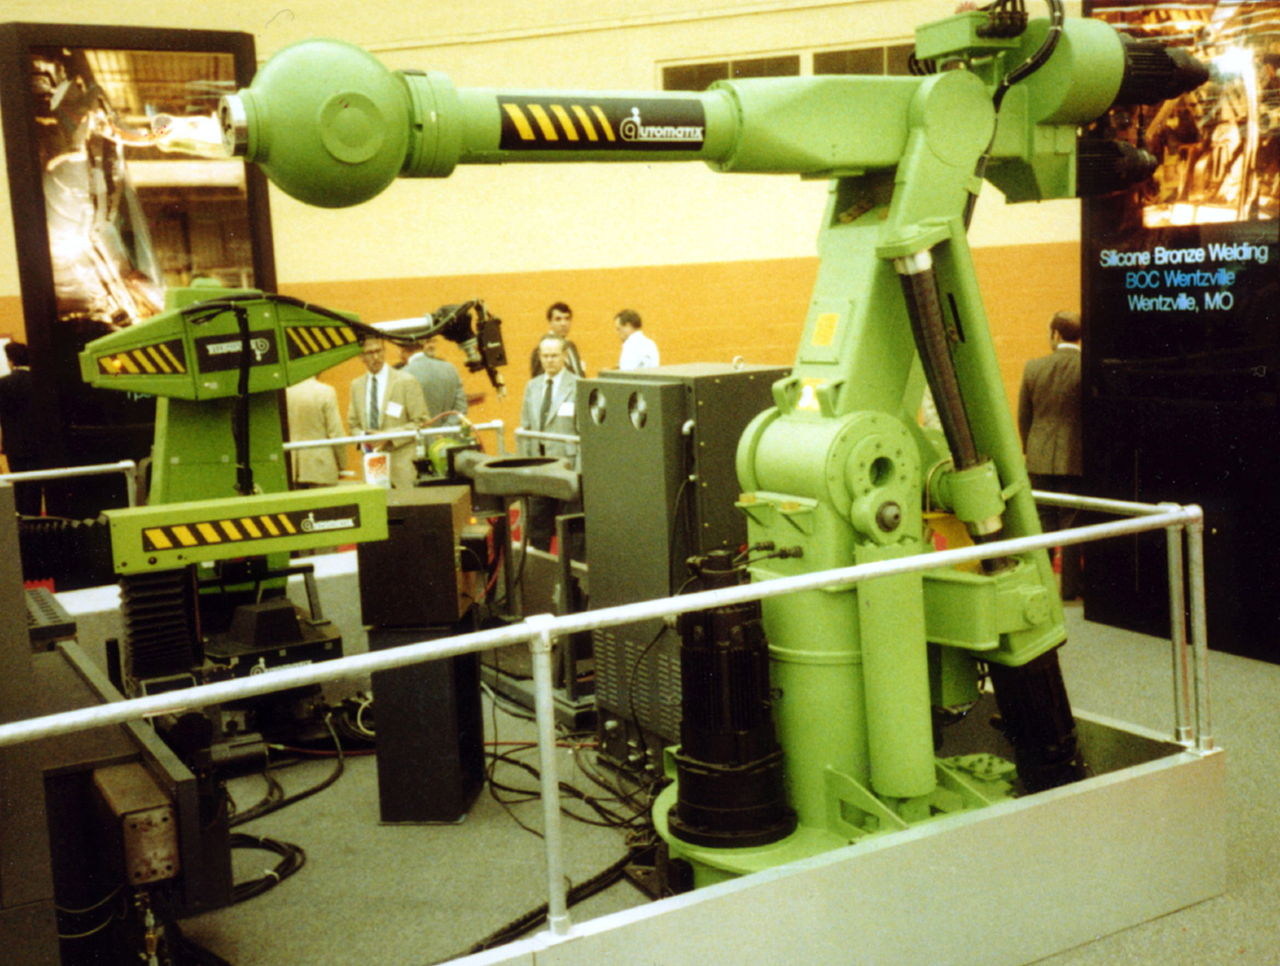
\includegraphics[width=\textwidth]{figures/Automatix.jpg}
			\copyright Wikipedia
		\end{column}
	\end{columns}
\end{frame}